% !Mode:: "TeX:UTF-8"

\chapter{国内外研究现状及分析}[Example]


\section{国外内研究现状}[Number]

国内外研究普遍采用的初生对流的定义是多普勒天气雷达首次检测到对流云反射率回波大于等于35dB。基于卫星资料的初生对流检测算法主要采用多普勒天气雷达检测的初生对流作为准则。利用卫星资料的初生对流检测方法主要采用的是传统的多通道阈值方法,通过对于不同波长的红外亮温通道的卫星图像进行判断。初生对流的检测的前提需要时序的对流检测以及对对流的跟踪。

基于卫星图像的传统对流识别方法主要是采用的阈值法\cite{覃丹宇2014利用静止气象卫星监测初生对流的研究进展},阈值法是最简单最常用的图像分割方法,通常适用于目标和背景差别明显的特征判识。对于卫星图像的长波红外通道,判定对流的采用的是红外亮温阈值,早期采用的方法有温度阈值、面积阈值和温度梯度阈值等。阈值法最大的问题是阈值的划定并不存在一个统一的标准,收到季节、海拔和经纬度的影响,不同地域的不同时间的阈值划分也应有所差异。从应用情况看,国内外相关的研究所采用的阈值通常在240K-250K之间。

基于卫星图像序列的传统对流目标的跟踪主要包括面积重叠法和统计法\cite{张春桂2017基于卫星和雷达资料的对流云团识别跟踪}。传统方法首先采用阈值法识别对流云团,根据亮温值连续低于某阈值进行判别利用云团轮廓码保存对流云团边界。采用多种阈值保存不同阈值下标注的对流云团结果。面积重叠法是假定对流云团不发生形变和旋转的前提下,利用连续两个时刻的对流云团边界计算对流云团的运动矢量。相重叠的面积越大,表明同一对流云团的可能性越高,再利用线性外推对对流云团进行预测,通过统计法的方法对生成的对流云团进行修正。

除了较为成熟的传统方法,对流外推本质是视频预测问题,初生对流的检测可以看作图像分割问题。图像语义分割方法以及视频预测方面的方法也能够对初生对流的检测给予很多启发性的方法。



\section{国内外文献综述及简析}[Index]
\subsection{基于自编码器的视频预测方法研究现状}

自编码器是一种以无监督的方式来学习数据表征的神经网络,通常用来做数据降维。自编码器通常分为编码器和解码器两部分,编码器将数据编码为潜在变量,解码器将潜在变量重建为原数据。自编码器有很多变体,例如降噪自编码器、稀疏自编码器、变分自编码器(VAE)。因为自编码器可以高效地进行数据降维,相当一部分视频预测模型采用了自编码器架构,如图~\ref{auto_encoder}~所示。

\begin{figure}[h]
	\centering
	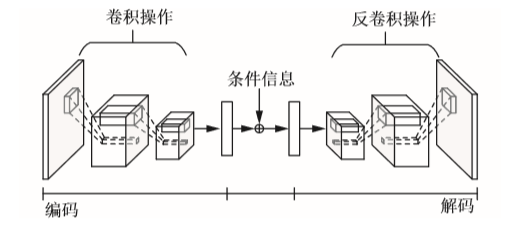
\includegraphics[width = 0.4\textwidth]{auto_encoder.png}
	\caption{基于自编码器的视频预测模型架构}
	\label{auto_encoder}
\end{figure}

自编码器架构下表现较好的是ConvLSTM,与LSTM不同,ConvLSTM在计算过程中用卷积操作代替了矩阵乘法,如公式~\ref{convLSTM}~所示,很好的利用卷积提取图像中的空间信息和利用LSTM提取时序信息。后来在ConvLSTM的基础上,又提出了训练代价更低,参数量更小的ConvGRU,在参数量和训练时间大大减少的前提下,精度能够得到基本保障。
\begin{equation}\label{convLSTM}
\begin{gathered}
$$
i_{t} = \sigma(W_{xi} \ast X_{t} + W_{hi} \ast H_{t-1} + W_{ci} \circ C_{t-1} + b_{i}) \\
f_{t} = \sigma(W_{xf} \ast X_{t} + W_{hf} \ast H_{t-1} + W_{cf} \circ C_{t-1} + b_{f})  \\
C_{t} = f_{t} \circ C_{t-1} + i_{t} \circ tanh(W_{xc} \ast X_{t} + W_{hc} \ast H_{t-1} + b_{c}) \\
o_{t} = \sigma(W_{xo} \ast X_{t} + W_{ho} \ast H_{t-1} + W_{oi} \circ C_{t-1} + b_{o})\\
H_{t} = o_{t} \circ tanh(C_{t})
$$
\end{gathered}
\end{equation}


